% The hard direction of the classical-price theorem: unsatisfiability reduced
% to drop safety. What to LOOK at is the mirror -- every gate of the compute
% block is undone by its partner in the uncompute block, so the scratch qubits
% reach the drop at |0>, and the ONE gate with no partner is the copy into the
% target, which is why the temporary reaches it holding B(x) and nothing else.
%
% Drawn for B = x1 AND NOT x2, which is two gates, so s = 2. The general shape
% is the same: one scratch qubit per gate of B, an AND becoming a Toffoli and
% a NOT becoming a CNOT followed by X.
%
% CONVENTIONS. The triangle and the descending bars are figures/criterion's:
% a triangle starts a register in a fixed state, the bars end one, and ending
% one is the drop. They are what marks the temporary here.
%
% REGISTER ORDER, and why it is not criterion's. That figure has two wires and
% puts the temporary on top. Here the temporary is BELOW the visible register,
% because with it on top every compute gate would have to reach from a visible
% wire, past the target, to a scratch wire: four connectors would cross the
% target's wire, and the Toffoli's target would sit between its two controls.
% The figure's whole claim is that one gate touches that wire. Drawn this way
% every gate has its controls above its target, exactly two connectors cross
% anything (the two Toffolis, over x2), and nothing crosses the target at all.
%
% Colour is not load-bearing: the copy gate is the only accent, and it is also
% the only gate in the corridor between the dashed blocks, the only gate below
% them, and the only mark on the target's wire.
%
% WIDTH. \textwidth is 395.8pt; this is about 365pt. The two notes carry an
% explicit text width, because it is those, not the circuit, that set the box.
%
%   make figures                                    compiles it
%   \includegraphics{figures/classical-price}       includes it
\documentclass[tikz,border=3pt]{standalone}
% ---------------------------------------------------------------------------
% figures/house.tex -- the shared look. Every figure \input's this, so six
% figures look like one hand drew them instead of six.
%
% HOW FIGURES WORK HERE. tikz/pgf is NOT on ACM's production package list, so
% the documents never load it. Each figure is its own standalone document in
% this directory, compiled to a PDF by `make figures`, and pulled into a
% section with
%
%     \begin{figure}
%       \centering
%       \includegraphics{figures/my-figure}
%       \caption{What to LOOK at, not what the figure is of.}
%       \label{fig:my-figure}
%     \end{figure}
%
% Three conventions:
%   * a float sits where it is discussed;
%   * a caption says what to look at, not what the figure is of;
%   * a figure is checked by rendering it and looking, not by a clean compile.
%
% The palette below is the same as the one in preamble.tex. It is repeated
% rather than shared because these are standalone documents that never see the
% paper's preamble, so a colour changed there must be changed here too.
% ---------------------------------------------------------------------------
\usepackage{amsmath}
% The figures build with LuaLaTeX like the documents, so their text is the
% paper's Libertine and their code is the paper's Iosevka.
\usepackage{fontspec}
\setmainfont{LinLibertine_R.otf}[BoldFont=LinLibertine_RB.otf,ItalicFont=LinLibertine_RI.otf,BoldItalicFont=LinLibertine_RBI.otf,Ligatures=TeX]
\setmonofont{Iosevka Custom}[Scale=MatchLowercase,RawFeature={-liga,-calt,-clig,-dlig}]
% Math in the figures is the paper's math: acmart sets Libertinus Math under
% LuaTeX, so the letters on a wire match the letters in the text around it.
\usepackage{unicode-math}
\setmathfont{LibertinusMath-Regular.otf}
\usetikzlibrary{positioning,arrows.meta,fit,backgrounds,calc}

% Blackboard Z, which the documents get from the paper preamble.
% Kept here so a figure never reaches for the paper's preamble.
\newcommand{\Z}{\mathbb{Z}}


\definecolor{ink}{HTML}{16191D}
\definecolor{accent}{HTML}{1F4E79}
\definecolor{accentsoft}{HTML}{E8EEF4}
% accent, accentwarm and accentplum mark the temporary's basis level -- level
% 0, 1, 2 -- wherever a picture or a matrix has to show which branch is which.
\definecolor{accentwarm}{HTML}{9A5B00}
\definecolor{accentplum}{HTML}{8E2F5F}
\definecolor{muted}{HTML}{5B6470}
\definecolor{hairline}{HTML}{C9CFD6}

\tikzset{
  % Every figure inherits this: thin lines, small type, generous air.
  house/.style={
    >={Stealth[length=2.1mm, width=1.6mm]},
    line width=0.5pt,
    node distance=9mm and 15mm,
    every node/.style={font=\small},
  },
  % A thing.
  box/.style={
    draw=ink, line width=0.5pt, rounded corners=1.5pt,
    inner xsep=6pt, inner ysep=4pt, align=center,
  },
  % A thing we are drawing attention to. One per figure, at most.
  boxhi/.style={box, draw=accent, fill=accentsoft, text=ink},
  % A thing that is context, not content.
  boxdim/.style={box, draw=hairline, text=muted},
  % An arrow, and the word on it.
  flow/.style={->, draw=ink},
  flowdim/.style={->, draw=hairline},
  lbl/.style={font=\footnotesize\itshape, text=accent, inner sep=2pt},
  lbldim/.style={font=\footnotesize, text=muted, inner sep=2pt},
  % A dashed grouping rectangle behind a set of nodes.
  group/.style={draw=hairline, dashed, rounded corners=2pt, inner sep=7pt},
}


% A control dot, a CNOT/Toffoli target, and the line joining them. Coordinates
% are plain numbers, so they are centimetres; radii carry their own units.
\newcommand{\ctl}[3][ink]{\fill[#1] (#2,#3) circle (1.35pt);}
\newcommand{\targ}[3][ink]{%
  \draw[#1, line width=0.5pt] (#2,#3) circle (1.7mm);
  \draw[#1, line width=0.5pt] (#2,{#3-0.17}) -- (#2,{#3+0.17});
  \draw[#1, line width=0.5pt] ({#2-0.17},#3) -- ({#2+0.17},#3);}
\newcommand{\vlink}[4][ink]{\draw[#1, line width=0.5pt] (#2,#3) -- (#2,#4);}
\newcommand{\nohyph}{\hyphenpenalty=10000 \exhyphenpenalty=10000}

\begin{document}
% gnd is figures/criterion's drop glyph, repeated here for the same reason the
% palette is: a standalone figure never reaches for another one's definitions.
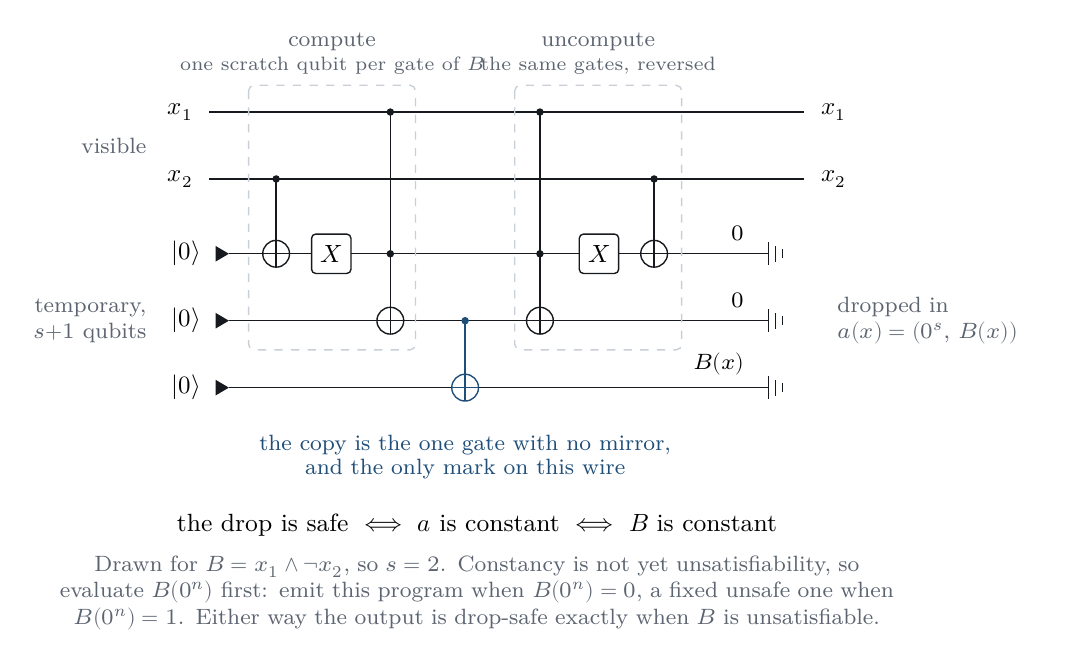
\begin{tikzpicture}[house,
  gnd/.pic={\draw[ink] (0,0) -- (0.10,0); \draw[ink] (0.10,0.145) -- (0.10,-0.145);
            \draw[ink] (0.19,0.100) -- (0.19,-0.100); \draw[ink] (0.28,0.055) -- (0.28,-0.055);}]

  % ---- the five wires -------------------------------------------------
  % Visible on top: x1 = 0, x2 = -0.85. Temporary below, set off by a wider
  % gap: c1 = -1.8, c2 = -2.65, t = -3.5.
  \foreach \y in {0,-0.85} { \draw[ink] (0,\y) -- (7.55,\y); }
  \node[anchor=east, font=\small] at (-0.08, 0)    {$x_1$};
  \node[anchor=east, font=\small] at (-0.08,-0.85) {$x_2$};
  \node[anchor=west, font=\small] at (7.65, 0)     {$x_1$};
  \node[anchor=west, font=\small] at (7.65,-0.85)  {$x_2$};

  \foreach \y in {-1.8,-2.65,-3.5} {
    \draw[ink] (0.25,\y) -- (7.0,\y);
    \fill[ink] (0.25,\y) ++(-0.17,-0.10) -- ++(0,0.20) -- ++(0.17,-0.10) -- cycle;
    \node[anchor=east, font=\small] at (0.02,\y) {$|0\rangle$};
    \pic at (7.0,\y) {gnd};
  }

  \node[lbldim, anchor=east] at (-0.72,-0.425) {visible};
  \node[lbldim, anchor=east, align=right] at (-0.72,-2.65) {temporary,\\$s{+}1$ qubits};

  % ---- compute: one scratch qubit per gate of B -----------------------
  % g1: CNOT x2 -> c1, then g2: X on c1, which together write NOT x2.
  \vlink{0.85}{-0.85}{-1.8}  \ctl{0.85}{-0.85}  \targ{0.85}{-1.8}
  \node[box, fill=white, minimum size=5mm, inner sep=1pt] at (1.55,-1.8) {$X$};
  % g3: Toffoli x1, c1 -> c2, which writes x1 AND (NOT x2) = B(x).
  \vlink{2.3}{0}{-2.65}  \ctl{2.3}{0}  \ctl{2.3}{-1.8}  \targ{2.3}{-2.65}

  % ---- copy: the one gate with no mirror ------------------------------
  \vlink[accent]{3.25}{-2.65}{-3.5}
  \ctl[accent]{3.25}{-2.65}  \targ[accent]{3.25}{-3.5}

  % ---- uncompute: the same gates, in reverse order --------------------
  \vlink{4.2}{0}{-2.65}  \ctl{4.2}{0}  \ctl{4.2}{-1.8}  \targ{4.2}{-2.65}
  \node[box, fill=white, minimum size=5mm, inner sep=1pt] at (4.95,-1.8) {$X$};
  \vlink{5.65}{-0.85}{-1.8}  \ctl{5.65}{-0.85}  \targ{5.65}{-1.8}

  % ---- the two blocks. Neither reaches the target's wire. --------------
  \draw[draw=hairline, dashed, rounded corners=2pt] (0.5,0.34) rectangle (2.62,-3.02);
  \draw[draw=hairline, dashed, rounded corners=2pt] (3.88,0.34) rectangle (6.0,-3.02);
  \node[lbldim, anchor=south, align=center] at (1.56,0.4)
    {compute\\[-1pt]\scriptsize one scratch qubit per gate of $B$};
  \node[lbldim, anchor=south, align=center] at (4.94,0.4)
    {uncompute\\[-1pt]\scriptsize the same gates, reversed};

  % ---- what reaches the drop ------------------------------------------
  \node[anchor=south east, font=\footnotesize] at (6.92,-1.76) {$0$};
  \node[anchor=south east, font=\footnotesize] at (6.92,-2.61) {$0$};
  \node[anchor=south east, font=\footnotesize] at (6.92,-3.46) {$B(x)$};
  \node[lbldim, anchor=west, align=left, text width=2.5cm,
        execute at begin node=\nohyph] at (7.9,-2.65)
    {dropped in \mbox{$a(x)=(0^{s},\,B(x))$}};

  % ---- the readoff ----------------------------------------------------
  \node[font=\footnotesize, text=accent, anchor=north, align=center] at (3.25,-3.98)
    {the copy is the one gate with no mirror,\\[-1pt]%
     and the only mark on this wire};
  \node[anchor=north, font=\small] at (3.4,-4.98)
    {the drop is safe $\iff$ $a$ is constant $\iff$ $B$ is constant};
  \node[lbldim, anchor=north, text width=10.8cm, align=center, font=\footnotesize,
        execute at begin node=\nohyph] at (3.4,-5.56)
    {Drawn for \mbox{$B = x_1 \wedge \lnot x_2$}, so \mbox{$s = 2$}. Constancy is
     not yet unsatisfiability, so evaluate \mbox{$B(0^{n})$} first: emit this
     program when \mbox{$B(0^{n}) = 0$}, a fixed unsafe one when
     \mbox{$B(0^{n}) = 1$}. Either way the output is drop-safe exactly when
     $B$ is unsatisfiable.};

\end{tikzpicture}
\end{document}
